\documentclass[a4paper]{article}

%================================================================================================================================
%
% Packages
%
%================================================================================================================================

\usepackage[T1]{fontenc} 	% pour caractères accentués
\usepackage[utf8]{inputenc}  % encodage utf8
\usepackage[french]{babel}	% langue : français
\usepackage{fourier}			% caractères plus lisibles
\usepackage[dvipsnames]{xcolor} % couleurs
\usepackage{fancyhdr}		% réglage header footer
\usepackage{needspace}		% empêcher sauts de page mal placés
\usepackage{graphicx}		% pour inclure des graphiques
\usepackage{enumitem,cprotect}		% personnalise les listes d'items (nécessaire pour ol, al ...)
\usepackage{hyperref}		% Liens hypertexte
\usepackage{pstricks,pst-all,pst-node,pstricks-add,pst-math,pst-plot,pst-tree,pst-eucl} % pstricks
\usepackage[a4paper,includeheadfoot,top=2cm,left=3cm, bottom=2cm,right=3cm]{geometry} % marges etc.
\usepackage{comment}			% commentaires multilignes
\usepackage{amsmath,environ} % maths (matrices, etc.)
\usepackage{amssymb,makeidx}
\usepackage{bm}				% bold maths
\usepackage{tabularx}		% tableaux
\usepackage{colortbl}		% tableaux en couleur
\usepackage{fontawesome}		% Fontawesome
\usepackage{environ}			% environment with command
\usepackage{fp}				% calculs pour ps-tricks
\usepackage{multido}			% pour ps tricks
\usepackage[np]{numprint}	% formattage nombre
\usepackage{tikz,tkz-tab} 			% package principal TikZ
\usepackage{pgfplots}   % axes
\usepackage{mathrsfs}    % cursives
\usepackage{calc}			% calcul taille boites
\usepackage[scaled=0.875]{helvet} % font sans serif
\usepackage{svg} % svg
\usepackage{scrextend} % local margin
\usepackage{scratch} %scratch
\usepackage{multicol} % colonnes
%\usepackage{infix-RPN,pst-func} % formule en notation polanaise inversée
\usepackage{listings}

%================================================================================================================================
%
% Réglages de base
%
%================================================================================================================================

\lstset{
language=Python,   % R code
literate=
{á}{{\'a}}1
{à}{{\`a}}1
{ã}{{\~a}}1
{é}{{\'e}}1
{è}{{\`e}}1
{ê}{{\^e}}1
{í}{{\'i}}1
{ó}{{\'o}}1
{õ}{{\~o}}1
{ú}{{\'u}}1
{ü}{{\"u}}1
{ç}{{\c{c}}}1
{~}{{ }}1
}


\definecolor{codegreen}{rgb}{0,0.6,0}
\definecolor{codegray}{rgb}{0.5,0.5,0.5}
\definecolor{codepurple}{rgb}{0.58,0,0.82}
\definecolor{backcolour}{rgb}{0.95,0.95,0.92}

\lstdefinestyle{mystyle}{
    backgroundcolor=\color{backcolour},   
    commentstyle=\color{codegreen},
    keywordstyle=\color{magenta},
    numberstyle=\tiny\color{codegray},
    stringstyle=\color{codepurple},
    basicstyle=\ttfamily\footnotesize,
    breakatwhitespace=false,         
    breaklines=true,                 
    captionpos=b,                    
    keepspaces=true,                 
    numbers=left,                    
xleftmargin=2em,
framexleftmargin=2em,            
    showspaces=false,                
    showstringspaces=false,
    showtabs=false,                  
    tabsize=2,
    upquote=true
}

\lstset{style=mystyle}


\lstset{style=mystyle}
\newcommand{\imgdir}{C:/laragon/www/newmc/assets/imgsvg/}
\newcommand{\imgsvgdir}{C:/laragon/www/newmc/assets/imgsvg/}

\definecolor{mcgris}{RGB}{220, 220, 220}% ancien~; pour compatibilité
\definecolor{mcbleu}{RGB}{52, 152, 219}
\definecolor{mcvert}{RGB}{125, 194, 70}
\definecolor{mcmauve}{RGB}{154, 0, 215}
\definecolor{mcorange}{RGB}{255, 96, 0}
\definecolor{mcturquoise}{RGB}{0, 153, 153}
\definecolor{mcrouge}{RGB}{255, 0, 0}
\definecolor{mclightvert}{RGB}{205, 234, 190}

\definecolor{gris}{RGB}{220, 220, 220}
\definecolor{bleu}{RGB}{52, 152, 219}
\definecolor{vert}{RGB}{125, 194, 70}
\definecolor{mauve}{RGB}{154, 0, 215}
\definecolor{orange}{RGB}{255, 96, 0}
\definecolor{turquoise}{RGB}{0, 153, 153}
\definecolor{rouge}{RGB}{255, 0, 0}
\definecolor{lightvert}{RGB}{205, 234, 190}
\setitemize[0]{label=\color{lightvert}  $\bullet$}

\pagestyle{fancy}
\renewcommand{\headrulewidth}{0.2pt}
\fancyhead[L]{maths-cours.fr}
\fancyhead[R]{\thepage}
\renewcommand{\footrulewidth}{0.2pt}
\fancyfoot[C]{}

\newcolumntype{C}{>{\centering\arraybackslash}X}
\newcolumntype{s}{>{\hsize=.35\hsize\arraybackslash}X}

\setlength{\parindent}{0pt}		 
\setlength{\parskip}{3mm}
\setlength{\headheight}{1cm}

\def\ebook{ebook}
\def\book{book}
\def\web{web}
\def\type{web}

\newcommand{\vect}[1]{\overrightarrow{\,\mathstrut#1\,}}

\def\Oij{$\left(\text{O}~;~\vect{\imath},~\vect{\jmath}\right)$}
\def\Oijk{$\left(\text{O}~;~\vect{\imath},~\vect{\jmath},~\vect{k}\right)$}
\def\Ouv{$\left(\text{O}~;~\vect{u},~\vect{v}\right)$}

\hypersetup{breaklinks=true, colorlinks = true, linkcolor = OliveGreen, urlcolor = OliveGreen, citecolor = OliveGreen, pdfauthor={Didier BONNEL - https://www.maths-cours.fr} } % supprime les bordures autour des liens

\renewcommand{\arg}[0]{\text{arg}}

\everymath{\displaystyle}

%================================================================================================================================
%
% Macros - Commandes
%
%================================================================================================================================

\newcommand\meta[2]{    			% Utilisé pour créer le post HTML.
	\def\titre{titre}
	\def\url{url}
	\def\arg{#1}
	\ifx\titre\arg
		\newcommand\maintitle{#2}
		\fancyhead[L]{#2}
		{\Large\sffamily \MakeUppercase{#2}}
		\vspace{1mm}\textcolor{mcvert}{\hrule}
	\fi 
	\ifx\url\arg
		\fancyfoot[L]{\href{https://www.maths-cours.fr#2}{\black \footnotesize{https://www.maths-cours.fr#2}}}
	\fi 
}


\newcommand\TitreC[1]{    		% Titre centré
     \needspace{3\baselineskip}
     \begin{center}\textbf{#1}\end{center}
}

\newcommand\newpar{    		% paragraphe
     \par
}

\newcommand\nosp {    		% commande vide (pas d'espace)
}
\newcommand{\id}[1]{} %ignore

\newcommand\boite[2]{				% Boite simple sans titre
	\vspace{5mm}
	\setlength{\fboxrule}{0.2mm}
	\setlength{\fboxsep}{5mm}	
	\fcolorbox{#1}{#1!3}{\makebox[\linewidth-2\fboxrule-2\fboxsep]{
  		\begin{minipage}[t]{\linewidth-2\fboxrule-4\fboxsep}\setlength{\parskip}{3mm}
  			 #2
  		\end{minipage}
	}}
	\vspace{5mm}
}

\newcommand\CBox[4]{				% Boites
	\vspace{5mm}
	\setlength{\fboxrule}{0.2mm}
	\setlength{\fboxsep}{5mm}
	
	\fcolorbox{#1}{#1!3}{\makebox[\linewidth-2\fboxrule-2\fboxsep]{
		\begin{minipage}[t]{1cm}\setlength{\parskip}{3mm}
	  		\textcolor{#1}{\LARGE{#2}}    
 	 	\end{minipage}  
  		\begin{minipage}[t]{\linewidth-2\fboxrule-4\fboxsep}\setlength{\parskip}{3mm}
			\raisebox{1.2mm}{\normalsize\sffamily{\textcolor{#1}{#3}}}						
  			 #4
  		\end{minipage}
	}}
	\vspace{5mm}
}

\newcommand\cadre[3]{				% Boites convertible html
	\par
	\vspace{2mm}
	\setlength{\fboxrule}{0.1mm}
	\setlength{\fboxsep}{5mm}
	\fcolorbox{#1}{white}{\makebox[\linewidth-2\fboxrule-2\fboxsep]{
  		\begin{minipage}[t]{\linewidth-2\fboxrule-4\fboxsep}\setlength{\parskip}{3mm}
			\raisebox{-2.5mm}{\sffamily \small{\textcolor{#1}{\MakeUppercase{#2}}}}		
			\par		
  			 #3
 	 		\end{minipage}
	}}
		\vspace{2mm}
	\par
}

\newcommand\bloc[3]{				% Boites convertible html sans bordure
     \needspace{2\baselineskip}
     {\sffamily \small{\textcolor{#1}{\MakeUppercase{#2}}}}    
		\par		
  			 #3
		\par
}

\newcommand\CHelp[1]{
     \CBox{Plum}{\faInfoCircle}{À RETENIR}{#1}
}

\newcommand\CUp[1]{
     \CBox{NavyBlue}{\faThumbsOUp}{EN PRATIQUE}{#1}
}

\newcommand\CInfo[1]{
     \CBox{Sepia}{\faArrowCircleRight}{REMARQUE}{#1}
}

\newcommand\CRedac[1]{
     \CBox{PineGreen}{\faEdit}{BIEN R\'EDIGER}{#1}
}

\newcommand\CError[1]{
     \CBox{Red}{\faExclamationTriangle}{ATTENTION}{#1}
}

\newcommand\TitreExo[2]{
\needspace{4\baselineskip}
 {\sffamily\large EXERCICE #1\ (\emph{#2 points})}
\vspace{5mm}
}

\newcommand\img[2]{
          \includegraphics[width=#2\paperwidth]{\imgdir#1}
}

\newcommand\imgsvg[2]{
       \begin{center}   \includegraphics[width=#2\paperwidth]{\imgsvgdir#1} \end{center}
}


\newcommand\Lien[2]{
     \href{#1}{#2 \tiny \faExternalLink}
}
\newcommand\mcLien[2]{
     \href{https~://www.maths-cours.fr/#1}{#2 \tiny \faExternalLink}
}

\newcommand{\euro}{\eurologo{}}

%================================================================================================================================
%
% Macros - Environement
%
%================================================================================================================================

\newenvironment{tex}{ %
}
{%
}

\newenvironment{indente}{ %
	\setlength\parindent{10mm}
}

{
	\setlength\parindent{0mm}
}

\newenvironment{corrige}{%
     \needspace{3\baselineskip}
     \medskip
     \textbf{\textsc{Corrigé}}
     \medskip
}
{
}

\newenvironment{extern}{%
     \begin{center}
     }
     {
     \end{center}
}

\NewEnviron{code}{%
	\par
     \boite{gray}{\texttt{%
     \BODY
     }}
     \par
}

\newenvironment{vbloc}{% boite sans cadre empeche saut de page
     \begin{minipage}[t]{\linewidth}
     }
     {
     \end{minipage}
}
\NewEnviron{h2}{%
    \needspace{3\baselineskip}
    \vspace{0.6cm}
	\noindent \MakeUppercase{\sffamily \large \BODY}
	\vspace{1mm}\textcolor{mcgris}{\hrule}\vspace{0.4cm}
	\par
}{}

\NewEnviron{h3}{%
    \needspace{3\baselineskip}
	\vspace{5mm}
	\textsc{\BODY}
	\par
}

\NewEnviron{margeneg}{ %
\begin{addmargin}[-1cm]{0cm}
\BODY
\end{addmargin}
}

\NewEnviron{html}{%
}

\begin{document}
\meta{url}{/exercices/loi-normale-estimation-bac-blanc-es-l-sujet-5-maths-cours-2018/}
\meta{pid}{10549}
\meta{titre}{Loi normale - Estimation - Bac blanc ES/L Sujet 5 - Maths-cours 2018}
\meta{type}{exercices}
%
\begin{h2}Exercice 1 (5 points)\end{h2}
\par
\textit{Les parties A et B sont indépendantes.}
\par
%============================================================================================================================
%
\TitreC{Partie A}
%
%============================================================================================================================
\par
La durée de vie, en heures, d'une lampe à incandescence peut être modélisée par une variable aléatoire $X$ qui suit la loi normale de moyenne $\mu =1\ 000$ et d'écart-type $\sigma = 200$.
\par
\begin{enumerate}
     \item
     Déterminer la probabilité que la durée de vie d'une lampe à incandescence soit supérieure à $1\ 400$ heures. On donnera une valeur approchée à $10^{-3}$ près.
     \item
     Déterminer la valeur du réel $m$, arrondie à la centaine, telle que :
     \[ p(X \geqslant m) = 0,16. \]
     \par
     Interpréter ce résultat dans le cadre de l'exercice.
     \item
     Parmi les quatre graphiques proposés ci-après, l'un d'eux représente la fonction de densité de probabilité associée à la loi normale de moyenne $\mu =1\ 000$ et d'écart-type $\sigma = 200$.
     \par
     \begin{center}
          \begin{extern}%width="600" alt="Graphique loi normale Proposition 1"
               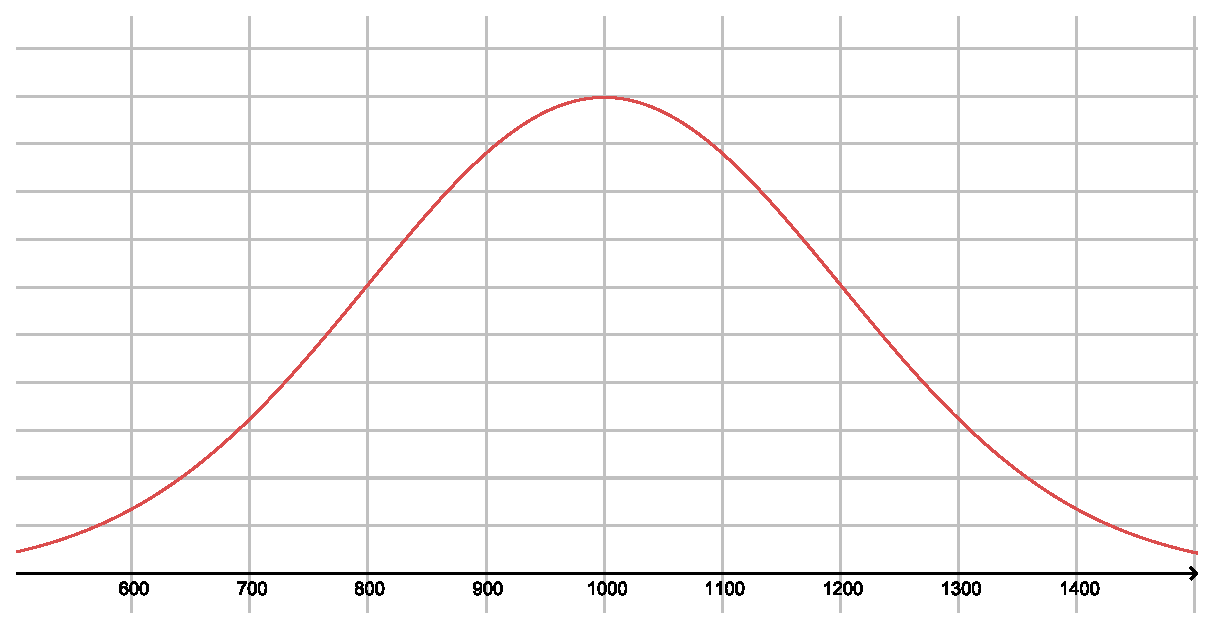
\includegraphics[width=0.9\textwidth]{images/BBESL-s5-1-1}% gbb 1 unite=1/100cm
          \end{extern}
     \end{center}
     \begin{center}
          Graphique 1.
     \end{center}
     \par
     \begin{center}
          \begin{extern}%width="600" alt="Graphique loi normale Proposition 2"
               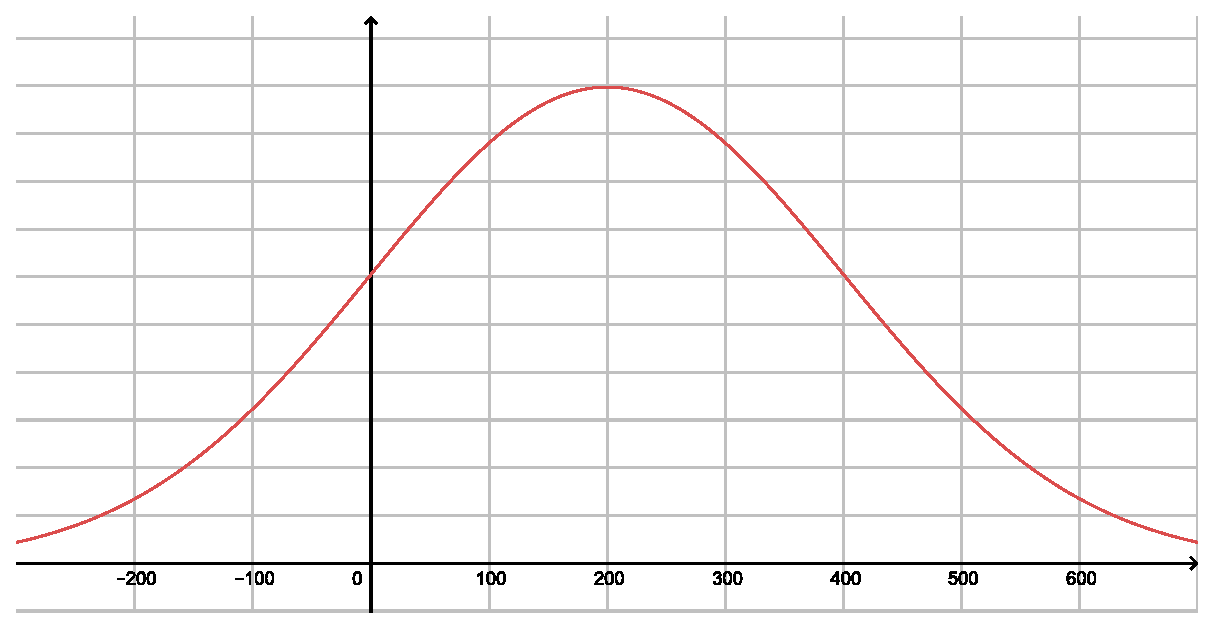
\includegraphics[width=0.9\textwidth]{images/BBESL-s5-1-2}% gbb 1 unite=1/100cm
          \end{extern}
     \end{center}
     \begin{center}
          Graphique 2.
     \end{center}
     \begin{center}
          \begin{extern}%width="600" alt="Graphique loi normale Proposition 3"
               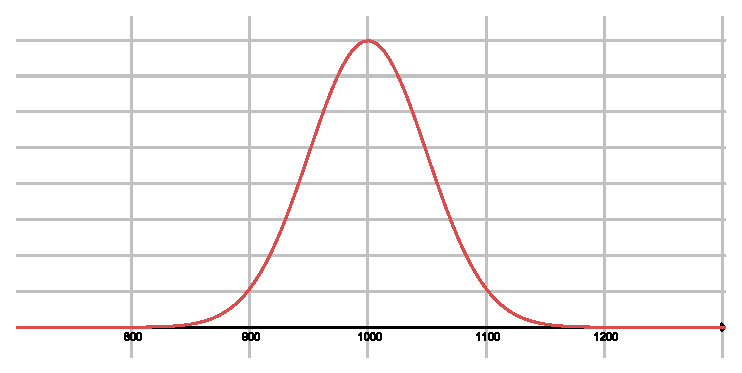
\includegraphics[width=0.9\textwidth]{images/BBESL-s5-1-3}% gbb 1 unite=1/100cm
          \end{extern}
     \end{center}
     \begin{center}
          Graphique 3.
     \end{center}
     \par
     \begin{center}
          \begin{extern}%width="600" alt="Graphique loi normale Proposition 4"
               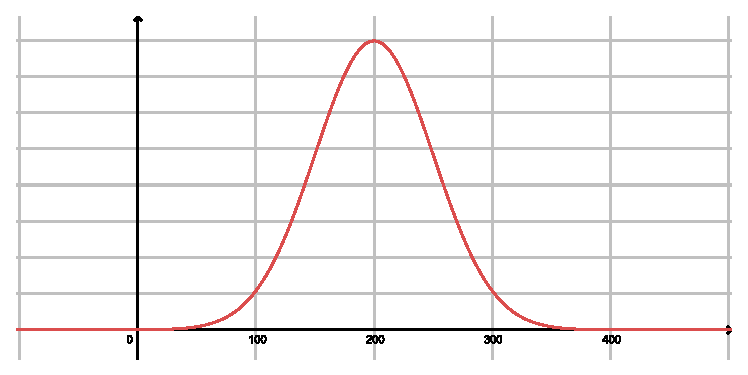
\includegraphics[width=0.9\textwidth]{images/BBESL-s5-1-4}% gbb 1 unite=1/100cm
          \end{extern}
     \end{center}
     \begin{center}
          Graphique 4.
     \end{center}
     \par
     Lequel ?
     \par
     Justifier votre réponse.
     \par
\end{enumerate}
\par
%============================================================================================================================
%
\TitreC{Partie B}
%
%============================================================================================================================
\par
Un fabriquant de lampes halogènes affirme que $75\%$ des lampes qu'il produit ont une durée de vie supérieure à 3\ 000 heures.
\par
Afin de vérifier cette affirmation, un laboratoire indépendant effectue un test sur 200 lampes choisies au hasard chez ce fabriquant.
\par
Il s'avère que seulement 140 d'entre elles ont une  durée de vie supérieure à 3\ 000 heures.
\par
\begin{enumerate}
     \item
     Déterminer, pour ce fabriquant, un intervalle de fluctuation asymptotique au seuil de $95\%$ de la proportion de lampes ayant une durée de vie supérieure à 3\ 000 heures pour un échantillon de taille 200.
     \item
     Les résultats du test mené par le laboratoire remettent-ils en cause l'affirmation du fabriquant ?
     \par
\end{enumerate}
\begin{corrige}
     %============================================================================================================================
     %
     \TitreC{Partie A}
     %
     %============================================================================================================================
     \par
     \begin{enumerate}
          \item %A1
          On cherche la probabilité de l'événement $(X>1~400)$.
          \par
          \`A la calculatrice, on trouve :
          \[ p(X>1~400) \approx 0,023\ \text{(au millième près)}. \]
          \par
          \item %A2
          On recherche la valeur du réel $m$ tel que :
          \[ p(X \geqslant m) = 0,16. \]
          \par
          \`A la calculatrice, on trouve :
          \par
          $m \approx 1200\ $ (arrondi à la centaine).
          \item %A3
          Le graphique correct est le \textbf{graphique 1.}
          \par
          La moyenne $\mu$ d'une loi binomiale correspond à l'abscisse du sommet de la courbe de Gauss.
          \par
          Cela permet d'éliminer immédiatement les graphiques \textbf{2.} et \textbf{4.} pour lesquels $\mu =200$.
          \par
          On sait que, pour une loi normale de moyenne $\mu$ et d'écart-type $\sigma$ :
          \[ p(\mu -\sigma \leqslant X \leqslant\mu +\sigma ) \approx 0,68. \]
          \par
          C'est à dire ici :
          \[ p(800 \leqslant X \leqslant 1\ 200 ) \approx 0,68 = 68\%. \]
          \par
          Or, $p(800 \leqslant X \leqslant 1\ 200$ représente l'aire, en unité d'aire, du domaine compris entre la courbe, l'axe des abscisses et les droites d'équations $x=800$ et $x=1\ 200$.
          \par
          Par ailleurs, l'aire totale du domaine compris entre la courbe et l'axe des abscisses vaut 1 unité d'aire.
          \par
          Pour le graphique \textbf{1.}, il est tout à fait raisonnable de penser que l'aire comprise entre les abscisses 800 et 1\ 200 représente 68\% de l'aire totale (\textit{voir figure ci-après}).
          \begin{center}
               \begin{extern}%width="600" alt="Graphique loi normale Solution 1"
                    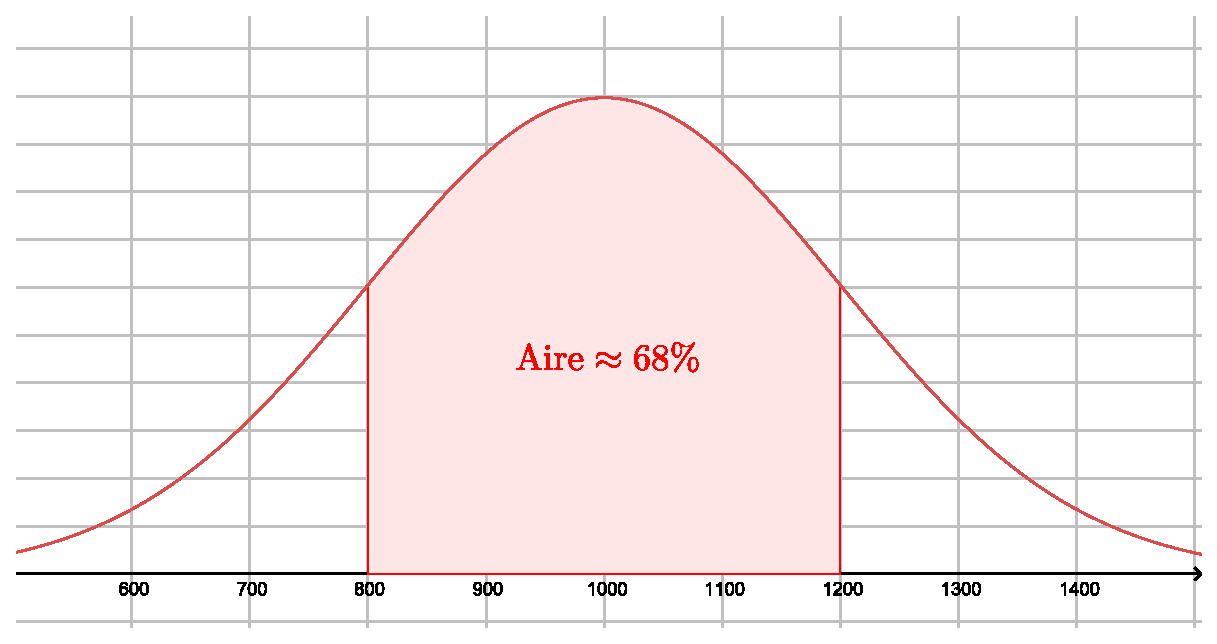
\includegraphics[width=0.9\textwidth]{images/BBESL-s5-1-5}% gbb 1 unite=1/100cm
               \end{extern}
          \end{center}
          \begin{center}
               Graphique 1.
          \end{center}
          \par
          Par contre, pour le graphique \textbf{3.}, l'aire comprise entre les abscisses 800 et 1\ 200 représente pratiquement 100\% de l'aire totale (\textit{voir figure ci-après}) ; ce graphique ne convient donc pas.
          \begin{center}
               \begin{extern}%width="600" alt="Graphique loi normale Solution 3"
                    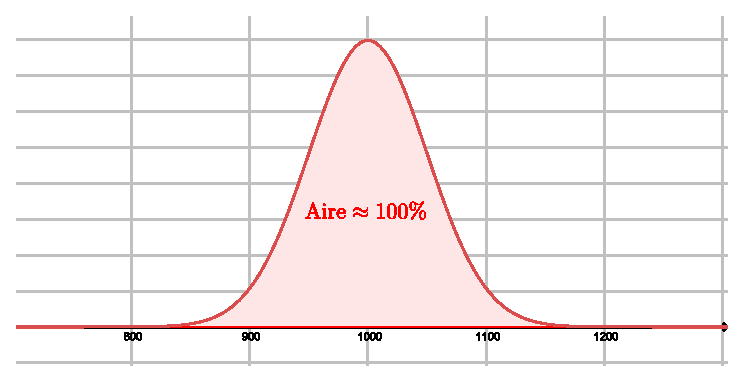
\includegraphics[width=0.9\textwidth]{images/BBESL-s5-1-6}% gbb 1 unite=1/100cm

\begin{center}
\imgsvg{BBESL-s5-1-6}{0.3}% alt="@" style="width:30rem"
\end{center}
               \end{extern}
          \end{center}
          \begin{center}
               Graphique 3.
          \end{center}
          \cadre{rouge}{À retenir}{
               Si la variable aléatoire $X$ suit une loi normale d'espérance $\mu$ et d'écart-type $\sigma$, alors :
               \par
               \begin{itemize}
                    \item  $p\left(\mu -\sigma \leqslant X\leqslant \mu + \sigma \right)\approx 0,68$ (à $10^{-2}$ près) ;
                    \item  $p\left(\mu -2\sigma \leqslant X\leqslant \mu + 2\sigma \right)\approx 0,95$ (à $10^{-2}$ près) ;
                    \item  $p\left(\mu -3\sigma \leqslant X\leqslant \mu + 3\sigma \right)\approx 0,997$ (à $10^{-3}$ près).
               \end{itemize}
          }
          \cadre{vert}{En pratique}{
               Pour une variable aléatoire $X$ qui suit une loi normale d'espérance $\mu$ et d'écart-type $\sigma$ :
               \par
               \begin{itemize}
                    \item  $\mu$ correspond à l'\textbf{abscisse du sommet} de la courbe ;
                    \item  plus l'écart-type $\sigma$ est grand, plus la \og cloche \fg{} est évasée ;
                    \item  environ \textbf{68\%} de l'aire située entre la courbe et l'axe des abscisses est comprise entre les abscisses $\mu - \sigma $ et $\mu + \sigma $.
               \end{itemize}
          }
     \end{enumerate}
     \par
     %============================================================================================================================
     %
     \TitreC{Partie B}
     %
     %============================================================================================================================
     \par
     \begin{enumerate}
          \item %B1
          D'après le fabriquant, la proportion théorique de lampes ayant une durée de vie supérieure à 3\ 000 heures est $p=0,75$.
          \par
          La taille  de l'échantillon est $n=200$.
          \par
          On vérifie que :
          \par
          \begin{itemize}
               \item $n=200 \geqslant 30$ ;
               \item $np=200 \times 0,75=150 \geqslant 5$ ;
               \item $n(1-p)=200 \times 0,25=50 \geqslant 5$.
          \end{itemize}
          \par
          Les conditions de validité étant remplies, l'intervalle cherché est :
          \par
          \[ I=\left[p-1,96\dfrac{\sqrt{p(1-p)}}{\sqrt{n}}~;~p+1,96\dfrac{\sqrt{p(1-p)}}{\sqrt{n}}\right]. \]
\medskip
          $p-1,96\dfrac{\sqrt{p(1-p)}}{\sqrt{n}}=0,75-1,96\dfrac{\sqrt{0,75(1-0,75)}}{\sqrt{200}}$
          \par
          $\phantom{p-1,96\dfrac{\sqrt{p(1-p)}}{\sqrt{n}}} \approx 0,690 $ (arrondi au millième).
          \par
          $p+1,96\dfrac{\sqrt{p(1-p)}}{\sqrt{n}}=0,75+1,96\dfrac{\sqrt{0,75(1-0,75)}}{\sqrt{200}}$
          \par
          $\phantom{p+1,96\dfrac{\sqrt{p(1-p)}}{\sqrt{n}}} \approx 0,810 $ (arrondi au millième).
          \par
          L'intervalle de fluctuation asymptotique au seuil de $95\%$ de la proportion de lampes ayant une durée de vie supérieure à 3\ 000 heures pour un échantillon de taille 200 est donc :
          \[ I=[0,69~;~0,81]. \]
          \cadre{rouge}{À retenir}{
               On note :
               \par
               \begin{itemize}
                    \item %
                    $n$ : la taille  de l'\textbf{échantillon},
                    \item %
                    $f$ : la fréquence du caractère dans l'\textbf{échan\-til\-lon},
                    \item %
                    $p$ : la proportion (connue ou supposée) du caractère dans la \textbf{population}.
               \end{itemize}
               \par
               Si les conditions $\bm{n\geqslant 30}$, $\bm{np\geqslant 5}$ et $\bm{n\left(1-p\right)\geqslant 5}$ sont vérifiées, l'intervalle de fluctuation asymptotique au seuil de 95\% est :
               \[  I=\left[ p-1,96\frac{\sqrt{p\left(1-p\right)}}{\sqrt{n}}~ ; ~p+1,96 \frac{\sqrt{p\left(1-p\right)}}{\sqrt{n}} \right]. \]
          }
          \item %B2
          Sur l'échantillon de 200 lampes, 140 ont une  durée de vie supérieure à 3\ 000 heures.
          \par
          Cela correspond à une fréquence observée de :
          \par
          $f=\dfrac{140}{200}=0,7$.
          \par
          Or $f=0,7$ appartient à l'intervalle de fluctuation $I$ trouvé à la question précédente.
          \par
          Au seuil de 95\%, les résultats du test \textbf{ne remettent pas en cause} l'affirmation du fabriquant.
          \cadre{vert}{En pratique}{
               En pratique, \textbf{pour valider ou rejeter une hypothèse} à l'aide d'un intervalle de fluctuation asymptotique :
               \begin{itemize}
                    \item %
                    On détermine l'intervalle de fluctuation asymptotique $I$ au seuil de 95\% en prenant pour $p$ la proportion \textbf{supposée} du caractère dans l'ensemble de la \textbf{population}.
                    \item %
                    On calcule la fréquence \textbf{observée} $f$ du caractère dans l'\textbf{échantillon}.
                    \item %
                    Si $f$ appartient à l'intervalle $I$ on \textbf{valide} l'hypothèse.
                    \item %
                    Si $f$ n'appartient pas à l'intervalle $I$ on \textbf{rejette} l'hypothèse. Le risque d'erreur en rejetant l'hypothèse est alors inférieur 5\%.
               \end{itemize}
          }
     \end{enumerate}
\end{corrige}

\end{document}